A continuación se realizará el análisis de las clases pertenecientes a la zona de datos. Como se ha explicado anteriormente en la sección \nameref{identificacion_subsistemas} perteneciente al capítulo \ref{chapter04}, la zona de datos incluye únicamente el subsistema de datos, que será el encargado de introducir datos en el sistema y devolverlos cuando sean pedidos por las visualizaciones.

La figura \ref{fig:clases_preliminares_modelo_book} muestra el diagrama de las clases preliminares de la zona datos.

\begin{landscape}
	\begin{figure}[ht]
		\centering
		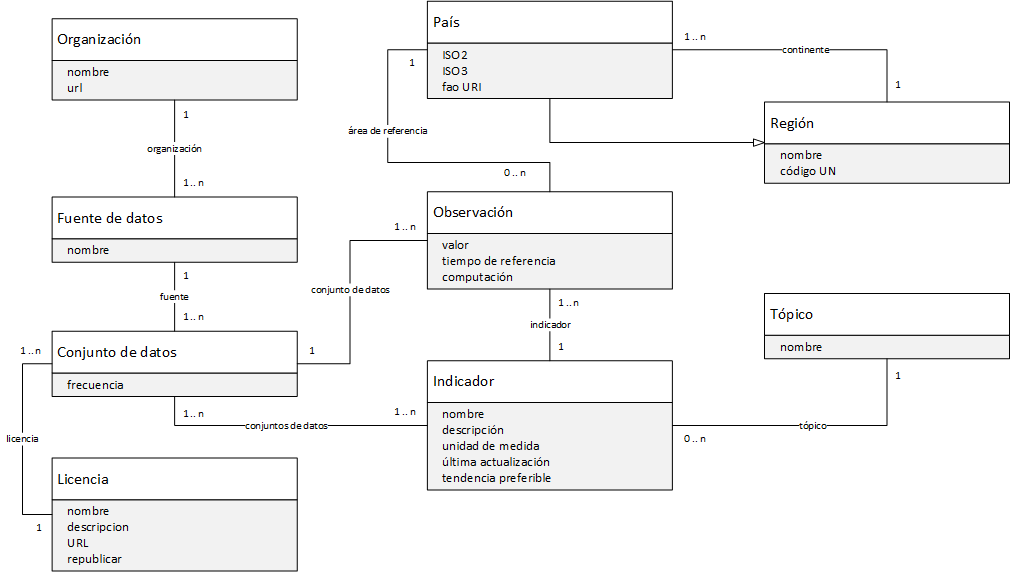
\includegraphics[]{clases/clases_book_preliminar}
		\caption{Diagrama de clases preliminares de la zona de datos}
		\label{fig:clases_preliminares_modelo_book}
	\end{figure}
\end{landscape}


\subsubsection{Descripción de las clases}
\begin{description}
\item[Región]	Representa un país o continente del mundo.  Sus atributos son los siguientes:
							\begin{itemize}
								\item \textbf{Nombre}  Será el nombre de la región, por ejemplo ``Europa'', ``África'' o ``España''.
								\item \textbf{Código UN}  Será el código numérico asignado por la División Estadística de las Naciones Unidas\footnote{Éste código recibe el nombre formal de ``ISO 3166-1 numeric''.  En \cite{un:standard-country-codes} y \cite{un:iso-3166-country-codes} puede encontrarse más información sobre éstos códigos.} para la región.
							\end{itemize}
\item[País]  Representa a un país del mundo sobre el que se almacenarán observaciones.  Además de los atributos de una región, sus atributos serán:
							\begin{itemize}
							\item \textbf{ISO2}  Será el código alfabético de dos letras asignado por la división estadística de las Naciones Unidas\footnote{Éste código recibe el nombre formal de ``ISO 3166-1 alpha-2''. Se utiliza para hacer representar países, territorios independientes o zonas geográficas de interés especial. En \cite{un:iso-3166-country-codes} puede encontrarse más información sobre éstos códigos} para el país.
							\item \textbf{ISO3}  Será el código alfabético de tres letras asignado por la división estadística de las Naciones Unidas\footnote{Éste código recibe el nombre formal de ``ISO 3166-1 alpha-3''. Se utiliza para hacer representar países, territorios independientes o zonas geográficas de interés especial. En \cite{un:iso-3166-country-codes} puede encontrarse más información sobre éstos códigos} para el país.  El código ISO3 consigue una mejor asociación con los nombres de los países que el código ISO2.
							\item \textbf{FAO URI}  Será la URI única del país en la Ontología Geopolítica de la Organización para la Alimentación y la Agricultura de las Naciones Unidas\footnote{La información sobre ésta ontología se encuentra disponible en \cite{fao:geopolitical-ontology}}.
							\item \textbf{Continente}  Representa el continente del que el país forma parte.  Cada país forma parte de un continente, pero un continente puede estar compuesto de muchos países.
							\end{itemize}
\item[Observación]  Representa una medición realizada en un tiempo concreto para un país determinado.  Las observaciones son utilizadas por las visualizaciones para presentar los datos de forma visual a los usuarios.  Sus atributos serán los siguientes:
							\begin{itemize}
							\item \textbf{Valor}  Será el valor concreto de la observación.
							\item \textbf{Tiempo de referencia}  Será el tiempo al que hace referencia la observación.  Por ejemplo, el tiempo de referencia puede ser un año, un mes, un intervalo de años, etc.
							\item \textbf{Computación}  Indica el tipo de computación de la que proviene la observación.  Por ejemplo indica si el valor de la observación es único o un agregado de los valores durante un determinado periodo de tiempo.
							\item \textbf{Área de referencia}  Representa el país al que la observación hace referencia.  Cada observación hace referencia a un país, pero un país puede tener muchas observaciones que le hagan referencia.
							\item \textbf{Indicador}  Representa el indicador al que pertenece la observación.  Cada observación pertenece a un indicador, pero un indicador puede contener multitud de observaciones.
							\item \textbf{Conjunto de datos}  Representa el conjunto de datos del que proviene la observación.  Cada observación proviene de un único conjunto de datos, pero cada conjunto de datos incluye múltiples observaciones.
							\end{itemize}
\item[Indicador]  Representa un elemento sobre el que se realizan observaciones.  Sus atributos son lo siguientes:
							\begin{itemize}
							\item \textbf{Nombre}  Es un nombre corto para un indicador.
							\item \textbf{Descripción}  Es una descripción sobre lo que representa el indicador.  Por ejemplo ``Índice de Desarrollo Humano''\footnote{El Índice de Desarrollo Humano (HDI) es un indicador real mantenido por el United Nations Development Programme (UNDP) y que se encontrará en la zona de datos del portal final}.
							\item \textbf{Unidad de medida}  Representa la unidad de medida de las observaciones del indicador.  Por ejemplo el indicador ``propiedad de las tierras por parte de mujeres'' podría tener una unidad de medida en porcentaje.
							\item \textbf{Última actualización}  Indica la fecha de la última actualización del indicador o alguna de sus observaciones en el sistema.
							\item \textbf{Tendencia preferible}  Representa si es preferible que el valor del indicador crezca o disminuya a lo largo del tiempo.  Por ejemplo para el indicador ``mortalidad infantil'' la tendencia preferible será que disminuya.
							\item \textbf{Tópico}  Representa el tópico (categoría) en la que se incluye el indicador.  Cada indicador pertenece a un tópico, pero un tópico puede tener muchos indicadores relacionados.
							\item \textbf{Conjuntos de datos}  Representa los conjuntos de datos en los que el indicador está presente.  Un indicador puede estar presente en muchos conjuntos de datos y, al mismo tiempo, un conjunto de datos puede contener muchos indicadores diferentes.
							\end{itemize}
\item[Tópico]  Representa un categoría de indicadores que tratan sobre un mismo tema.  Sus atributos son lo siguientes:
							\begin{itemize}
							\item \textbf{Nombre}  Es el nombre del tópico.  Por ejemplo ``Tierra y género'' o ``Propiedad de la tierra''.
							\end{itemize}
\item[Conjunto de datos]  Representa un conjunto de datos que se inserta en el sistema.  Sus atributos son los siguientes:
							\begin{itemize}
							\item \textbf{Frecuencia}  Indica la frecuencia con la que se actualiza el conjunto de datos.  Algunas frecuencias de ejemplo pueden ser: ``anual'', ``trimestral'', etc.
							\item \textbf{Fuente}  Representa la fuente de la que proviene el conjunto de datos.  Cada conjunto de datos pertenece a una fuente, pero cada fuente puede contener varios conjuntos de datos.
							\item \textbf{Licencia}  Representa la licencia bajo la que se publica el conjunto de datos.  Cada conjunto de datos se publica bajo una licencia, pero cada licencia puede tener varios conjuntos de datos.
							\end{itemize}
\item[Licencia]  Representa una licencia bajo la que se publica un conjunto de datos.  Sus atributos son los siguientes:
							\begin{itemize}
							\item \textbf{Nombre}  Es el nombre corto de la licencia,  Por ejemplo  ``CC BY 2.0''.
							\item \textbf{Descripción}  Es una descripción larga sobre el funcionamiento de la licencia.
							\item \textbf{URL}  Será la URL bajo la que se encuentra disponible la información de la licencia  Por ejemplo \url{https://creativecommons.org/licenses/by/2.0/} para la licencia ``CC BY 2.0''.
							\item \textbf{Republicar}  Indica si la licencia permite republicar los contenidos o no.
							\end{itemize}
\item[Fuente de datos] Representa una fuente de datos de la que se extraen conjuntos de datos.  Sus atributos son los siguientes:
							\begin{itemize}
							\item \textbf{Nombre}  Es el nombre de la fuente de datos.  Por ejemplo ``Indicadores sobre el hambre''.
							\end{itemize}
\item[Organización]  Representa una organización que provee fuentes y conjuntos de datos que se importan en el sistema:
							\begin{itemize}
							\item \textbf{Nombre}  Es el nombre de la organización.  Por ejemplo  ``The Statistics Division of the FAO''\footnote{\url{http://faostat.fao.org/}}.
							\item \textbf{URL}  Es la URL del sitio web de la organización.
							\end{itemize}
\end{description}